\chapter{Discretization of a convection-diffusion problem}

%\long\def\COMMENT#1{\par\vbox{\hrule\vskip1pt \hrule width.125in height0ex #1\vskip1pt\hrule}}


\label{chap-conv}
\section{Introduction}
This chapter concerns convection-diffusion equations of the form: 
\begin{eqnarray*}
-\mu\Delta u + v\cdot \nabla u  &=& f \quad \textrm{in}\ \Omega\\
u&=& g \quad \textrm{on}\ \partial\Omega
\end{eqnarray*}
Here $v$ is  typically a velocity, $\mu$ is the diffusivity,  and $u$ is the 
unknown variable of interest. We assume the Dirichlet condition $u=g$ on 
the boundary, while $f$ is a source term.  

The problem is a singular perturbation problem. That is, the problem is well-posed for $\mu > 0$ but becomes over--determined as $\mu$ tends to zero. For $\mu=0$ the Dirichlet conditions should only be set on the inflow domain $\Gamma$; that is, where $n \cdot v < 0$ for the outward unit normal $n$. 

For many practical situations $\mu>0$, but small in the sense that $\mu \ll |v|$. For such problems, the solution 
will often be similar to the solution of the reduced problem with $\mu=0$ except close to the 
non-inflow boundary $\partial \Omega \backslash \Gamma$. Here, there will typically be a boundary layer $\exp{(\|v\|_\infty x / \mu)}$.      
Furthermore, discretizations often shows unphysical oscillations starting at this boundary layer.    

The next example shows a 1D convection diffusion problem resulting in non-physical oscillations due to the use
of a standard Galerkin approximation. 

\begin{example}{\textbf{Standard Galerkin approximation}} \label{ex1} \\
Consider the following 1D problem convection diffusion problem, where $v=-1$ for simplicity: 
\begin{eqnarray}
-u_x - \mu u_{xx} = 0, \\ 
u(0) = 0, u(1) = 1 . 
\end{eqnarray}
The analytical solution is: 
\[
u(x) = \frac{e^{-x/\mu} - 1}{e^{-1/\mu} - 1}. 
\]
Hence, for $\mu \rightarrow 0$ , both $e^{-x/\mu}$ and $e^{-1/\mu}$ 
will be small and $u(x) \approx 1$ unless $x\approx 0$. However, close to the 
outflow boundary at $x=0$, there will be a boundary layer where $u$ has exponential growth. 

We solve the problem with a standard Galerkin method using linear first
order Lagrange elements. To be specific, the variational problem is: \\    
Find $u \in H^1_{(0,1)}$ such that 
\[
\int_0^1 -u_x v + \mu u_x v_x \dx   = 0, \quad \forall v \in H^1_{(0,0)} .  
\]
Here, $H^1_{(0,1)}$ contains functions $u\in H^1$ with $u=0$ at $x=0$ and $u=1$ and $x=1$, while
$H^1_{(0,0)}$ contains functions that are zero both at $x=0$ and $x=1$. We
consider a $\mu=0.01$, a relatively large $\mu$, to enable us to see the
differences on a relatively coarse mesh.     

\begin{figure}
\begin{center}
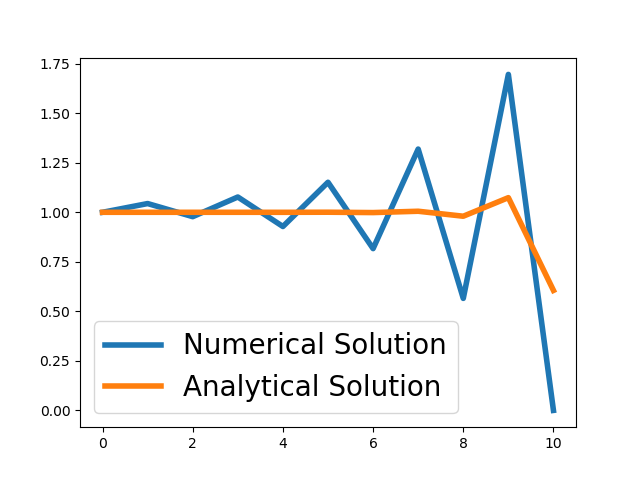
\includegraphics[width=0.45\textwidth]{chapters/conv-diff/plots/conv-diff.png}
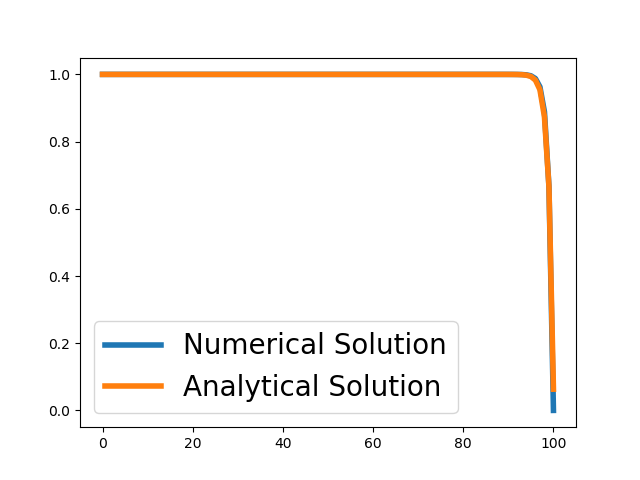
\includegraphics[width=0.45\textwidth]{chapters/conv-diff/plots/conv-diff-hr.png}
\caption{Solution of the convection diffusion problem obtained with 10 and 100 elements. 
The left figure obtained on a mesh with 10 elements shows wild oscillations, while the 
mesh with 100 elements demonstrate a nicely converged solution.}
\label{fig:conv1}
\end{center}
\end{figure}

Both the numerical and analytical solutions are shown in Figure \ref{fig:conv1}. Clearly, 
the numerical solution is polluted by non-physical oscillations on the coarse
mesh with 10 elements, while a good approximation is obtained for 100 elements.     


Finally, we show the complete code for this example: 
\begin{python}
from dolfin import *
for N in [10, 100]:

  mesh = UnitInterval(N)
  V = FunctionSpace(mesh, "CG", 1)

  u = TrialFunction(V)
  v = TestFunction(V)

  mu_value = 1.0e-2 
  mu = Constant(mu_value)
  f = Constant(0)
  h = mesh.hmin()

  a = (-u.dx(0)*v + mu*u.dx(0)*v.dx(0))*dx  
  L = f*v*dx  

  u_analytical = Expression("(exp(-x[0]/e) - 1)/ (exp(-1/%e) - 1)" % (mu_value, mu_value))  
  def boundary(x):
      return x[0] < DOLFIN_EPS or x[0] > 1.0 - DOLFIN_EPS

  bc = DirichletBC(V, u_analytical, boundary) 

  U = Function(V)
  solve(a == L, U, bc) 

  U_analytical = project(u_analytical, V)

  import pylab 
  pylab.plot(U.vector().array())
  pylab.plot(U_analytical.vector().array())
  pylab.legend(["Numerical Solution", "Analytical Solution"])
  pylab.show()
\end{python}
$\square$ 
\end{example}

To understand Example \ref{ex1} we first remark that the discretization corresponds to the following 
central finite difference scheme: 
\begin{eqnarray*}
-\frac{\mu}{h^2}\left[u_{i+1}-2u_i+u_{i-1}\right] - 
\frac{v}{2h}\left[u_{i+1}-u_{i-1}\right] &=& 0, \quad i=1,\ldots,N-1\\
u_0=0,\quad u_N=1 &&
\end{eqnarray*}
Above, we kept $v$ as a variable such that we may discuss the directionality of upwinding in terms of the convection. 
Clearly, if $\mu=0$ then the scheme reduces to  
\begin{eqnarray*}
-\frac{v}{2h}\left[u_{i+1}-u_{i-1}\right] &=& 0, \quad i=1,\ldots,N-1\\
u_0=0,\quad u_N=1 &&
\end{eqnarray*}
Here, it is clear that $u_{i+1}$ is coupled to $u_{i-1}$, but not to 
$u_{i}$. 
Hence, this scheme allow for an alternating
sequence of $u_{i+1}=u_{i-1}=\ldots$, while $u_{i}=u_{i-2}=\ldots$
resulting in oscillations. 

One cure for these oscillations is upwinding. That is, instead
of using a central difference scheme, we employ the following difference
scheme:   
\begin{eqnarray*}
\frac{du}{dx} (x_i) = \frac{1}{h}[u_{i+1}-u_{i}] \quad   \mbox{ if } \ v < 0, \\ 
\frac{du}{dx} (x_i) = \frac{1}{h}[u_{i}-u_{i-1}] \quad  \mbox{ if } \ v > 0 .  
\end{eqnarray*}
Using this scheme, oscillations will disappear. The approximation will however only be first order.

There is a relationship between upwinding and artificial diffusion.  If we discretize $u_x$ with a central difference and add diffusion as $\epsilon =h/2 \Delta $ we get
\begin{eqnarray*}
 \frac{u_{i+1}  -  u_{i-1}}{2 h}    &  \textrm{central scheme, first order derivative}  \\
+ \frac{h}{2} \, \frac{-u_{i+1}   + 2 u_{i}    -u_{i-1}}{h^2}  &  \textrm{central scheme, second order derivate}   \\
= \frac{u_{i} -u_{i-1}}{h} &  \textrm{upwind scheme}   
\end{eqnarray*}

\noindent
Hence, upwinding is equivalent to adding artificial diffusion with $\epsilon=h/2$; that is, in both cases we actually solve the problem
\[-(\mu+\epsilon)u_{xx} + vu_x = f.\]
using a central difference scheme. 

Finite difference upwinding is difficult to express using finite elements methods, but
it is closely to adding some kind of diffusion to the scheme.  
The next example shows the solution of the problem in Example \ref{ex1} with 
artificial diffusion added. 

\begin{example}{\textbf{Stabilization using artificial diffusion}} \label{cd:ex2} \\
Consider again the following 1D problem convection diffusion problem: 
\begin{eqnarray}
-u_x - \mu u_{xx} = 0, \\ 
u(0) = 0, u(1) = 1 . 
\end{eqnarray}

We solve the problem with a standard Galerkin method using linear first
order Lagrange elements as before, but we add artificial diffusion. To be specific, the variational problem is:  \\   
Find $u \in H^1_{(0,1)}$ such that 
\[
\int_0^1 -u_x v + (\mu + \beta h) u_x v_x = 0, \quad \forall v \in H^1_{(0,0)},    
\]
where $\beta=0.5$ corresponds to the finite difference scheme with artificial diffusion mentioned
above.  Below is the code for the changed variational form:

\begin{python}
  beta_value = 0.5 
  beta = Constant(beta_value)
  f = Constant(0)
  h = mesh.hmin()
  a = (-u.dx(0)*v + mu*u.dx(0)*v.dx(0) + beta*h*u.dx(0)*v.dx(0))*dx  
\end{python}

\begin{figure}
\begin{center}
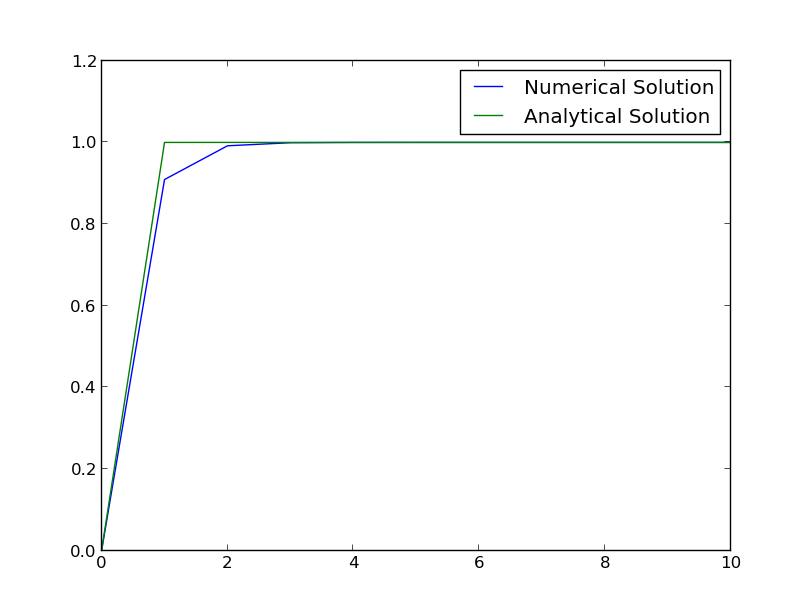
\includegraphics[width=6cm]{chapters/conv-diff/plots/conv-diff-stab.png}
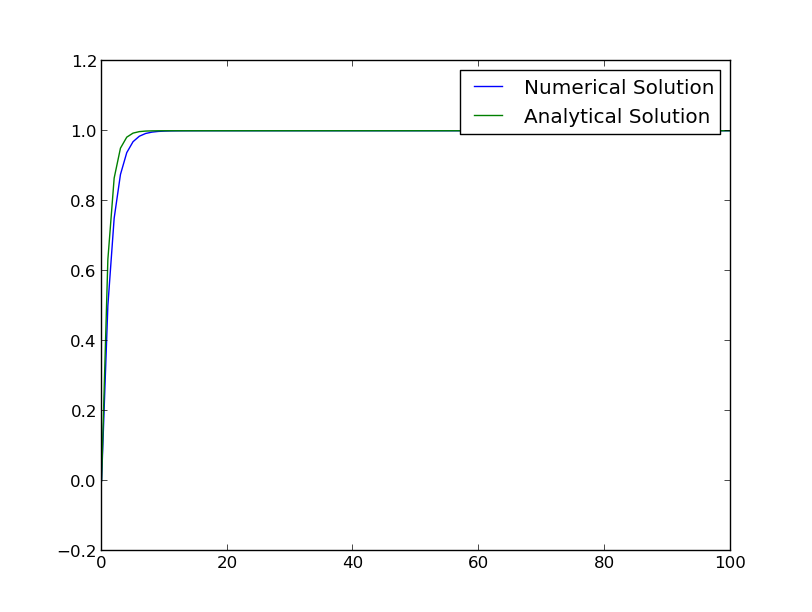
\includegraphics[width=6cm]{chapters/conv-diff/plots/conv-diff-hr-stab.png}
\caption{Solution of the convection diffusion problem obtained with 10 and 100 elements
using artificial diffusion to stabilize.}
\label{fig:conv2}
\end{center}
\end{figure}

Figure \ref{fig:conv2} shows the solution for 10 and 100 elements when using artificial diffusion 
stabilization.  Clearly, the solution for the coarse grid has improved dramatically since the
oscillations have vanished and the solution appear smooth. It is, however, interesting to note
that the solution for the fine mesh is actually less accurate than the solution in Fig \ref{fig:conv2} 
for the corresponding fine mesh. The reason is that the scheme is now first order, while the 
scheme in Example \ref{ex1} is second order.    
\end{example}



\section{Streamline diffusion/Petrov-Galerkin methods}
In the previous section we saw that artificial diffusion may be added to convection diffusion dominated problems to avoid 
oscillations. The diffusion was, however, added in a rather ad-hoc manner.  
Here, we will see how diffusion may be added in a consistent way; 
that is, without changing the solution as $h\rightarrow 0$. 
This leads us to streamline diffusion using the Petrov-Galerkin method.
Our problem reads: \\ 
Find $u$ such that 
\begin{eqnarray*}
-\mu\Delta u + v\cdot\nabla u &=& f \quad \textrm{in}\ \Omega, \\
u&=& g \quad \textrm{on}\ \partial\Omega .
\end{eqnarray*}
The \textbf{weak formulation} reads: \\
Find $u\in H_g^1$ such that 
\[
a(u,w) = b(w) \quad \forall\ w\in H_0^1, 
\]
where
\begin{eqnarray*}
a(u,w) &=& \int_\Omega\mu\nabla u \cdot \nabla w \dx + \int_\Omega v \cdot \nabla uw \dx,   \\
b(w) &=& \int_\Omega fw \dx . 
\end{eqnarray*}
Here, $H_g^1$ is the subspace of $H^1$ where the trace equals $g$ on the boundary $\partial \Omega$.  

The \textit{standard Galerkin} discretization is: \\
Find $u_h\in V_{h,g}$ such that 
\begin{equation}
\label{Galerkin}
a(u_h, v_h) = (f,v_h)\ \forall v_h\in V_{h,0}.
\end{equation}
Here, $V_{h,g}$  and $V_{h,0}$ are the subspaces with traces that equals $g$ and $0$ on 
the boundary, respectively.  

Adding artificial diffusion 
to the standard Galerkin discretization, 
as was done in Example \ref{cd:ex2}, 
can be done as: \\ 
Find $u_h\in V_{h,g}$ such that 
\[
a(u_h, v_h) + \frac{h}{2}(\nabla u_h, \nabla v_h)  = (f,v_h)\ \forall v_h\in V_{h,0}.
\]
Let
\[
\tau(u, v_h) =  a(u_h, v_h) - (f,v_h). 
\]
Then the \emph{truncation error} is first order in $h$; that is, 
\[
\tau(u) = \sup_{v \in V_h, v \not = 0} \frac{\tau (u, v_h)}{\|v\|_{V}} \sim \mathcal{O}(h). 
\]
Hence, the scheme is \emph{consistent} in the sense that 
\[
\lim_{h\rightarrow 0} \tau (u) \rightarrow 0 .  
\]
However, it is not \emph{strongly consistent} in the sense that $\tau(u) = 0$ for every
discretization, which is what is obtained with the Galerkin method due
to Galerkin-orthogonality:   
\[
\tau(u, v_h) =  a(u_h, v_h) - (f,v_h) = a(u_h - h, v_h) = 0 \quad \forall v_h \in V_h. 
\]


The \textit{Streamline diffusion/Petrov-Galerkin} method introduces a strongly consistent  
diffusion by employing alternative test functions. Let us therefore
assume that we have a space of test functions $W_h$.   
Abstractly, the Petrov-Galerkin method appears very similar to the Galerkin method, that is: \\ 
Find $u_h\in V_{h,g}$ such that 
\[
a(u_h, v_h) = (f,v_h) \quad \forall v_h\in W_{h,0}.
\]
Again, $V_{h,g}$  and $W_{h,0}$ are the subspaces with traces that equals $g$ and $0$ on 
the boundary, respectively.  
Notice that the only difference from the standard Galerkin formulation is that test and trial functions differ. 

On matrix form, the standard Galerkin formulation reads: 
\begin{equation}
A_{ij} = a(N_i, N_j ) = \int_\Omega\mu\nabla N_i \cdot \nabla N_j \dx + \int_\Omega v \cdot \nabla N_iN_j \dx, 
\label{eq:wGalerkin_A}
\end{equation}
while for the Petrov Galerkin method, we use the test functions $L_j$: 
\[A_{ij} = a(N_i, L_j ) = \int_\Omega\mu\nabla N_i \cdot \nabla L_j \dx + \int_\Omega v \cdot \nabla N_iL_j \dx\]
A clever choice of $L_j$ will enable us to add diffusion in a consistent way. To make sure
that the matrix is still quadratic, we should however make sure that the dimension of 
$V_h$ and $W_h$ are equal. 

Let $L_j$ be defined as $L_j = N_j + \beta h \, v\cdot\nabla N_j$. Writing out the matrix $A_{ij}$ in \eqref{eq:wGalerkin_A} now gives
\begin{eqnarray*}
A_{ij} &=& a(N_i, N_j + \beta h \, v\cdot\nabla N_j )\\
&=& \int_\Omega\mu\nabla N_i\cdot\nabla (N_j + \beta h \,  v\cdot\nabla N_j) \dx + \int_\Omega v \cdot \nabla N_i\cdot (N_j + \beta h \, v\cdot\nabla N_j) \dx\\
&=&\underbrace{
\int_\Omega\mu\nabla N_i \cdot \nabla N_j \dx + \int_\Omega v \cdot \nabla N_i\, N_j \dx}_
{\textrm{standard Galerkin}}
\\
&&\lefteqn{
+\underbrace{
\beta h \, \int_\Omega\mu\nabla N_i\cdot\nabla(v \cdot \nabla N_j) \dx
}_
{=0\ \textrm{third order term,  for linear elements}}+
\underbrace{\beta h \, \int_\Omega (v\cdot\nabla N_i) (v\cdot\nabla N_j) \dx}
_{\textrm{Artificial diffusion in $v$ direction}}
}
\end{eqnarray*}

Notice that also the righthand side changes
\[b(L_j) = \int_\Omega fL_j \dx = \int_\Omega f(N_j + \beta h \, v\cdot\nabla N_j) \dx\]
Thus, both the matrix and the righthand side are changed such that artificial diffusion is added in a consistent way. 

We summarize this derivation by stating the SUPG problem. 
Find $u_{h,sd}\in H_g^1$ such that 
\begin{equation}
\label{SUPG} 
a_{sd} (u,w) = b_{sd}(w) \quad \forall w\in H_0^1, 
\end{equation}
where
\begin{eqnarray*}
a_{sd}(u,w) &=& \int_\Omega\mu\nabla u \cdot \nabla w \dx + \int_\Omega v \cdot \nabla uw \dx \\
            &+& \beta h \,  \int_\Omega (v\cdot\nabla u) (v\cdot \nabla w) \dx  + \beta h \,  \mu \sum_e \int_{\Omega_e} -\Delta u (v\cdot\nabla w) \dx ,  \\
b_{sd} (w) &=& \int_\Omega fw \dx + \beta h \, \int_\Omega f v \cdot \nabla w \dx . 
\end{eqnarray*}



\section{Well posedness of the continuous problem}
Before we discuss error estimates of the discrete problem, we
briefly describe the properties of the continuous problem. 

\begin{theorem}{\textbf{Lax-Milgram theorem}} \\
Let $V$ be a Hilbert space, $a(\cdot, \cdot)$ be 
a bilinear form, $L(\cdot)$ a linear form, and let the following three conditions be satisfied: 
\begin{enumerate}
\item $a(u,u) \ge \alpha \|u\|^2_V, \quad \forall u \in V$,  \label{LM1} 
\item $a(u,v) \le C \|u\|_V \|v\|_V, \quad \forall u, v \in V$,  \label{LM2} 
\item $L(v) \le D \| v \|_V, \quad \forall v \in V$ .  \label{LM3} 
\end{enumerate}
Then the problem: Find $u\in V$ such that 
\[
a(u,v) = L(v) \quad \forall v \in V. 
\]
is well-posed in the sense that there exists a unique solution with the following 
stability condition
\[
\|u \|_V \le \frac{C}{\alpha} \|L\|_{V^*} .  
\]
\end{theorem}
Condition \eqref{LM1} is often refereed to as coersivity or positivity, while
\eqref{LM2} is called continuity or boundedness. Condition \ref{LM3} simply
states that the right-hand side should be in the dual space of $V$.    

In the following we will use Lax-Milgram's theorem to show that the convection-diffusion problem is well-posed. 
The Lax-Milgram's theorem is well-suited since it does not require symmetry of the bilinear form. 


We will only consider the homogeneous Dirichlet conditions in the current 
argument\footnote{Has the argument for reducing non-homogeneous Dirichlet conditions
to homogeneous Dirichlet conditions been demonstrated elsewhere?}.   
From Poincare's lemma we know  that 
\[
\|u\|_0 \le C_\Omega |u|_1.  
\]
Using Poincare, it is straightforward to show that the 
semi-norm     
\[
|u|_1 = (\int (\nabla u)^2   \dx)^{1/2}  
\]
and the standard $H^1$ norm 
\[
\|u \|_1  = (\int (\nabla u)^2 + u^2  \dx)^{1/2}  
\]
are equivalent. Hence, on $H^1_0$ the $|\cdot|_1$ is a norm
equivalent the $H^1$-norm. Furthermore, this norm will be easier to 
use for our purposes.  

For the convection-diffusion problem, we will consider two cases 1) incompressible flow, where
$\nabla \cdot v = 0 $ and 2) compressible flow, where $\nabla \cdot v \not = 0 $.  
Let us for the begin with the incompressible case.  
Further, let 
\begin{eqnarray*}
b(u,w) &=& \int_\Omega\mu\nabla u\nabla w \dx\\
c_v(u,w) &=& \int_\Omega v \cdot \nabla u \,w \dx\\
a(u,w) &=& a(u,w) + b(u,w)\\
\end{eqnarray*}
Furthermore, assuming for the moment that $u \in H^1_g, w\in H^1_0$, we have  
\begin{eqnarray*}
c_v(u,w) &=& \int_\Omega v\cdot \nabla u\, w \dx  \\ 
         &=&-\int_\Omega v\cdot \nabla w \, u \dx 
- \underbrace{\int_\Omega \nabla \cdot v \, u \, w \dx}_{= 0 \textrm{ (incompressibility)}} 
+ \underbrace{\int_\Gamma u \, w \, v \cdot n}_{ = 0  \textrm{ (Dirichlet conditions)}} \\       
         &=& - c_v(w,u) . 
\end{eqnarray*}
and therefore $c_v(\cdot, \cdot)$ is skew-symmetric. Letting $w=u$ we obtain that   
$c_v(u,u) = -c_v(u,u)$, which means that $c_v(u,u)=0$. 
Therefore, the first condition in Lax-Milgram's theorem \eqref{LM1} is satisfied:   
\[  
a(u,u) = b(u,u) \ge \mu |u|_1^2 .  
\]

The second condition, the boundedness of $a$ \eqref{LM2}, follows by applying Cauchy-Schwartz inequality
if we assume bounded flow velocities $\|v\|_{\infty}$.  
\begin{eqnarray*}
a(u,v) &=& \int_\Omega\mu\nabla u\nabla w \dx + \int_\Omega v\nabla uw \dx\\
       &\le& \mu |u|_1 |w|_1  + \|v\|_{\infty} |u|_1 \|w\|_0 \\   
       &\le& (\mu + \|v\|_{\infty} C_\Omega )  |u|_1 |v|_1 .    
\end{eqnarray*}

The third condition simply means that the right-hand side needs to be in the dual 
space of $H^1_g$. Hence, we obtain the following bounds by Lax-Milgram's theorem:   
\[
|u|_1 \le \frac{ \mu + C_\Omega \|v\|_{\infty}}{\mu} \|f\|_{-1} . 
\]
Notice that for convection-dominated problems $ C_\Omega \|v\|_{\infty} \gg \mu$ 
and the stability constant will therefore be large. 

In the case where $\nabla \cdot v \not = 0$, we generally obtain that $c_v(u,u) \not = 0$. 
To ensure that $a(u,u)$ is still positive, we must then put some restrictions on 
the flow velocities. That is, we need    
\[
|c_v(u,u)| \le a(u,u) .  
\]
If $C_\Omega \|v\|_\infty \le D \mu$ with $D < 1$ we obtain   
\begin{eqnarray*}
a(u,u) &=& \int_\Omega\mu\nabla u\nabla u \dx + \int_\Omega v\nabla uu \dx\\
       &\ge & \mu |u|_1 |v|_1  - \|v\|_{\infty} |u|_1 \|u\|_0 \\   
       &\ge& (\mu - \|v\|_{\infty} C_\Omega )  |u|_1 |u|_1 \\    
       &\ge& (\mu (1-D))  |u|_1^2 .    
\end{eqnarray*}
Further, the second condition of Lax-Milgram's theorem still applies.   
However, that $C_\Omega \|v\|_\infty \le D \mu$ is clearly very restrictive 
compared to the incompressible case.   

We remark that the Lax-Milgram conditions in the presence of the SUPG clearly will not 
be satisified in the continuous case because of the third order term
$ -\Delta u (v\cdot\nabla w)$. With this term, the second condition of Lax-Milgram is not satisified
with $C \le \infty$.  

Finally, in order to make the  
term $c_v(u,u)$ skew-symmetric, it was required that 
the boundary integral $\int_\Gamma u^2 \, w  \cdot n $ was zero.  
This was a consequence of the Dirichlet conditions. 
 In general, this is neither needed nor possible
at Neumann boundaries. As long as $\int_\Gamma u^2 \, w \cdot n \ge 0 $, the above argumentation is valid. From a 
physical point of view this means that there is outflow at the Neumann boundary, i.e., that $w\cdot n \ge 0$.  

\section{Error estimates}

Finally, we provide some error estimates for the
Galerkin method and the SUPG method applied to the
convection-diffusion equation. Central in the derivation
of both results are the following interpolation result.   


\begin{theorem}{\textbf{Approximation by interpolation}}\\
There exists an interpolation operator $I_h: H^{t+1} \rightarrow V_h$ 
where $V_h$ is a piecewise polynomial field of order $t$ with the property that   
for any $u\in H^t(\Omega)$ 
\[
\| u - I_h u \|_m \le  B h^{t+1-m} \|u\|_{t+1}  .  
\]
\end{theorem}
\begin{proof} %FIXME, this dose not look good
The bounds on the interpolation error is provided by 
the Bramble-Hilbert lemma for $t\ge 1$  and Clement's result (the case $t=1$), 
cf. e.g.~\cite{braess2007finite, brenner2008mathematical}.  
\end{proof}

For the Galerkin method the general and elegant result of Cea's lemma
provide us with error estimates. Cea's lemma applies to general 
conforming approximations, i.e. when $V_h \subset V$. In our
case $V=H_0^1(\Omega)$ and $V_h$ is a finite element subspace such 
as for example  a discretization in terms of the Lagrange elements (of any order). Hence, in our case 
$\|\cdot\|_V= |\cdot|_1$ and the $H^1$ semi-norm is equivalent with the full 
$H^1$ norm due to Poincare's inequality. 

\begin{theorem}{\textbf{Cea's lemma}} \\
Suppose the conditions for Lax-Milgram's theorem is satisfied and that
we solve the linear problem \eqref{Galerkin} on a finite element space
of order $t$. Then,     
\[
\|u-u_h\|_V     \le C_1 \frac{C B}{\alpha}  h^{t} \|u\|_{t+1}.   
\]
Here $C_1 = \frac{C B}{\alpha}$, where $B$ comes from the approximation property 
and $\alpha$ and $C$ are the constants of Lax-Milgram's theorem.    
\end{theorem}

\begin{proof}
The proof is straightforward and follows from the Galerkin orthogonality: 
\[
a(u - u_h, v) = 0, \quad \forall v \in V_h 
\]
Since $V_h \subset V$: 
\begin{eqnarray*}
\alpha \|u-u_h\|^2_{V} &\le& a(u-u_h, u-u_h)    \\ 
 &=& a(u-u_h, u-v) - a(u-u_h, v-u_h) \\ 
 &\le& C \|u-u_h\|_V \| u-v\|_V  .      
\end{eqnarray*}
Since $v-u_h\in V_h$. Furthermore,  $v$ is arbitrary and we may therefore choose $v = I_h u$ and obtain:  
\[
	|u-u_h|_1 \le \frac{C}{\alpha} |u - I_h u|_1 \le  \frac{CB}{\alpha} h^{t} \|u\|_t,   
\]
where $t-1$ is the order of the polynomials of the finite elements. 
\end{proof}

We remark, as mentioned above, that 
$\frac{C}{\alpha}$ is large for convection dominated problems and that this is what
causes the poor approximation on the coarse grid, shown in Example \ref{ex1}.  


To obtain improved error estimates for the SUPG method, we introduce  
an alternative norm: 
\begin{equation}
\label{supg:norm}
\|u\|_{sd} = \left(h\|v\cdot\nabla u\|^2 +  \mu |\nabla u|^2\right)^{1/2}
\end{equation}


\begin{theorem}
Suppose the conditions for Lax-Milgram's theorem is satisfied 
in the Hilbert space defined by the SUPG norm \eqref{supg:norm}
and that
we solve the SUPG problem \eqref{SUPG} on a finite element space
of order $1$. Then,  
\[\|u-u_h\|_{sd} \le Ch^{3/2}\|u\|_{2}\]
\end{theorem}

\begin{proof}
The proof can be found in e.g. \cite{elman2014finite, quarteroni2008numerical}. 
\end{proof}

\section{Exercises}

\begin{exercise}
Show that the matrix obtained from a central difference scheme applied to 
the operator $L u = u_x$ is skew-symmetric. Furthermore, show that
the matrix obtained by linear continuous Lagrange elements are also 
skew-symmetric. Remark: The matrix is only skew-symmetric in the  interior
of the domain, not at the boundary.    
\end{exercise}

\begin{exercise}
Estimate numerically the constant in Cea's lemma for various $\alpha$ and $h$ for the  Example \ref{ex1}. 
\end{exercise}

\begin{exercise}
Implement the problem $u=sin(\pi x)$, and $f = -\alpha u_{xx} - u_x$ and 
estimate numerically the constant in Cea's lemma for various $\alpha $.       
Compare with the corresponding constant estimated from Example \ref{ex1}. 
\end{exercise}


\begin{exercise}
Implement the problem $u=sin(\pi x)$, and $f = -\alpha u_{xx} - u_x$ using
SUPG and estimate the constants in the error estimate obtained by 
both the $|\cdot|_1$ and  the $\| \cdot \|_{v}$      
norms. 
Compare with the corresponding constant estimated from Example \ref{ex1}. 
\end{exercise}

 
 
\begin{exercise}
Investigate whether the coersivity condition holds when a 
homogeneous Neumann condition is assumed on the outflow. 
You may assume that $v\cdot n > 0$.   
\end{exercise}

\begin{exercise}
Consider the eigenvalues of the operators, 
$L_1$, $L_2$, and $L_3$, where
$L_1 u = u_x$, $L_2 u = -\alpha u_{xx}$, $\alpha=1.0e^{-5}$, 
and $L_3 = L_1 + L_2$, with homogeneous Dirchlet conditions. 
For which of the operators are the eigenvalues positive and
real? Repeat the exercise with $L_1 = x u_x$.   
\end{exercise}


\begin{exercise}
Compute the Soblev norms $\|\cdot\|_m$ of the function $sin(k \pi x)$ on 
the unit interval. Assume that the Soblev norm is $\|u\|_m = (-\Delta^m u, u)^{1/2}$.     
What happens with negative $m$? You may use either Fourier transformation or 
compute (eigenvalues of) powers of the stiffness matrix. 
\end{exercise}

\begin{exercise}
Perform numerical experiments to determine the order of approximation with respect 
to various Soblev norms and polynomial orders for the function  
$sin(k \pi x)$ on 
the unit interval.
\end{exercise}






%\section{Further reading}
%Further discussions on the convection-diffusion equation can be 
%found in, e.g.,\cite{elman2005finite, johnson2009numerical, quarteroni2008numerical}.  


